\begin{tikzpicture}[every node/.style={font=\footnotesize}]
  \draw[MidnightBlue,thick,->] (-7.4,0) -- (4.15,0);
  \draw[BurntOrange,line width=2.4pt] (-2.07,-0.16) -- (2.07,-0.16);
  \fill[BurntOrange] (-2.07,-0.16) circle (1.5pt);
  \fill[BurntOrange] (2.07,-0.16) circle (1.5pt);
  \fill[MidnightBlue] (-5.42,0) circle (2.4pt);
  \fill[BrickRed] (2.07,0) circle (2.6pt);
  \fill[black] (0,0) circle (1.5pt);
  \draw[MidnightBlue] (-2.07,0.10) -- (-2.07,-0.10);
  \node[MidnightBlue,anchor=south,align=center] at (-5.42,0.28) {$-\dfrac{1}{\sqrt{5}\,(1-\psi x)}$};
  \node[BrickRed,anchor=south,align=center] at (2.07,0.28) {$\dfrac{1}{\sqrt{5}\,(1-\varphi x)}$};
  \node[MidnightBlue,anchor=north] at (-5.42,-0.22) {$1/\psi\approx -1.618$};
  \node[BrickRed,anchor=north] at (2.07,-0.42) {$1/\varphi\approx 0.618$};
  \node[MidnightBlue,anchor=north] at (-2.07,-0.34) {$-1/\varphi$};
  \node[black,anchor=south] at (0,0.16) {$0$};
  \node[align=center] at (-1.6,-2.15) {$\displaystyle\frac{x}{(1-\varphi x)(1-\psi x)}=\frac{1}{\sqrt{5}}\left(\frac{1}{1-\varphi x}-\frac{1}{1-\psi x}\right)$};
\end{tikzpicture}
